\documentclass{article}
\usepackage[a4paper, total={7.5in, 10.5in}]{geometry}
\usepackage{multicol}
\usepackage{graphicx}
\usepackage{float}
\usepackage{tcolorbox}
\usepackage{verbatim}
\usepackage{soul}

\newcommand{\optimisation}[1]{
  \input{./assets/optimisations/#1.tex}
}

\begin{document}

\title{Assessed Exercise 1: Microarchitecture Optimisation in Splay Trees}
\author{Charlie Lidbury}
\maketitle

\begin{multicols}{2}

  \section{Intro}
  This report aims to roughly follow the structure of the specification, starting with the fixed exploration and then finishing with the energy optimization challenge. Apologies for the US English throughout, I can't figure out how to change my spell-check.

  \section{Studying Microarchitectural Effects}
  At the start of the specification, there are a few direct questions, this section answers those.

  \subsection{Parameters Interact (RUU vs LSQ vs Energy/IPC)}

  The more RUU you give the CPU, the more instructions per clock you get, likely because it can better utilize functional units, as shown in Figure \ref{fig:ipc_energy_vs_ruu}.

  \begin{figure}[H]
    \centering
    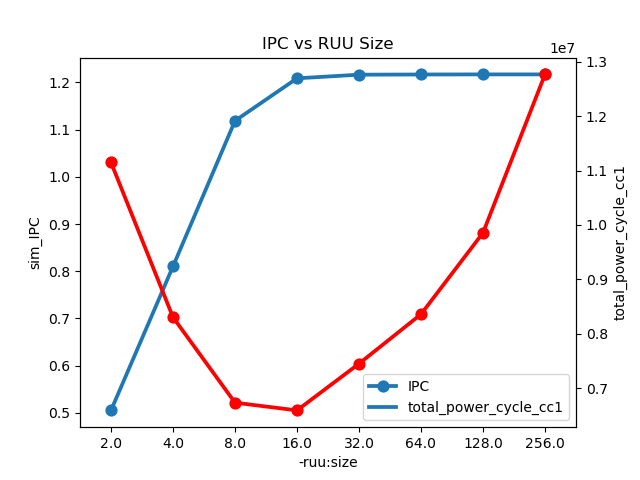
\includegraphics[width=\linewidth]{./assets/ipc_vs_ruu_size.png}
    \caption{IPC/Energy vs RUU Size}
    \label{fig:ipc_energy_vs_ruu}
  \end{figure}

  However, as shown by the red line, this does not translate to better energy efficiency forever. This is likely because the extra instructions per clock are not worth the extra energy cost of the larger RUU.

  If we vary both the RUU size and LSQ size at the same time, we can see that if either gets too small, the other becomes the bottleneck.

  \begin{figure}[H]
    \centering
    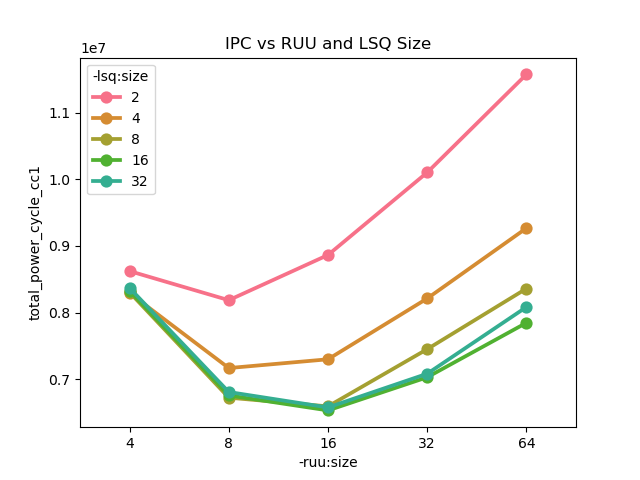
\includegraphics[width=\linewidth]{./assets/energy_vs_ruu_and_lsq_size.png}
    \caption{Energy vs RUU Size/LSQ Size}
    \label{fig:energy_vs_ruu_lsq}
  \end{figure}

  In Figure \ref{fig:energy_vs_ruu_lsq}, when the LSQ size is small, say 2, the optimal RUU size is 8. This is because the LSQ is the bottleneck, so the extra RUU space can't be utilized and it's just wasted energy. When there is more LSQ space, higher RUU numbers provide benefits.

  \subsection{Bottlenecks}
  Something is a bottleneck if increasing its size would speed up overall performance, so to investigate which components are bottlenecks, we can vary their size and see if it affects performance.

  We can alter the size/quantity of most components, but I'll assume for this question only the RUU and LSQ are under investigation.

  The default parameters are RUU=16 and LSQ=8, so I'll start there and increase. SimpleScalar doesn't seem to record simulated time, so I will assume that microarchitectural changes don't affect clock speed, and therefore the number of cycles is a good proxy for time.

  \begin{figure}[H]
    \centering
    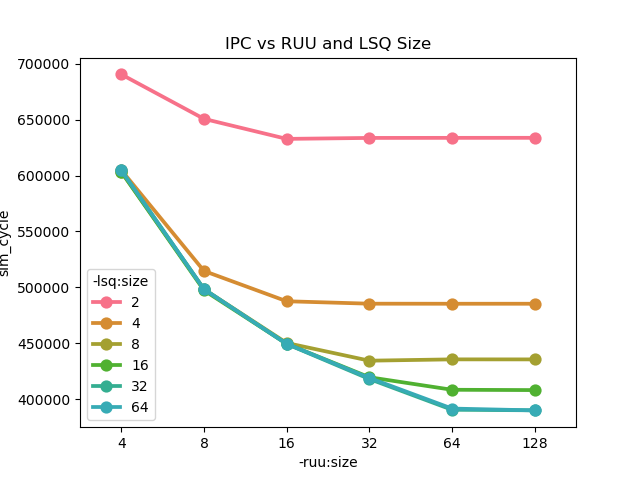
\includegraphics[width=\linewidth]{./assets/ruu_and_lsq_vs_sim_time.png}
    \caption{RUU and LSQ Increases vs performance}
    \label{fig:ruu_or_lsq_bottleneck}
  \end{figure}

  As shown in Figure \ref{fig:ruu_or_lsq_bottleneck}, which one is the bottleneck depends on the size of the other. If the RUU is small, the LSQ is the bottleneck, and vice versa.

  At the default parameters (RUU=16, LSQ=8) the LSQ seems to be the bottleneck because increasing the RUU past its default value of 16 doesn't increase performance. This is likely because the program has a lot of loads and stores, creating lots of entries in the LSQ.

  \subsection{Race-to-Finish Doesn't Always Win}
  As shown in Figure \ref{fig:energy_vs_ruu_lsq}, the RUU/LSQ configuration with the lowest energy usage in RUU=16, LSQ=16, Figure \ref{fig:ruu_or_lsq_bottleneck} shows the optimal configuration for instructions per clock it \textit{at least} RUU=128, LSQ=64. Although there are diminishing returns, it looks like increasing the RUU and LSQ size always results in faster runtime.

  \section{Minimising Total Energy}
  \subsection{Methodology}
  % Get program-specific knowledge
  % Use that to come up with reasonable parameters
  % Use systematic search to make sure we're in a local minimum
  My search for the optimal parameters will occur in two main stages:

  \textbf{Informed Optimisation} In the first section, I will reason about the program to find a set of reasonable variables; for instance, because I know there are very few floating point operations in the C source code, I can reduce the number of those to 1 without worrying too much about its implications on the other functional units.

  \textbf{Systematic Optimisation} In this section, I will use pure statistical search to make sure I'm in a local minimum. After this, there could still be other places in the parameter space with better performance, but I will at least know that any valid change to any parameter will result in performance degradation.

  % \subsection{Program Analysis}
  % In this section, I will discuss the various microarchitecture parameters we can adjust, and how they will likely affect the execution of the given splay tree program.

  % 

  % \subsubsection{Cache}
  % \label{analysis:cache}
  % The simulator allows us to adjust everything about the L1 and L2 cache (sets, block size, associativity, replacement strategy), as well as how many levels are unified between instructions and data.

  % 


  % Perhaps this will mean we won't need as big a cache, as we will get a large hit rate?


  % \subsubsection{Functional Units}
  % We can control how many integer/floating point ALUs/multipliers we have.

  % 

  % \subsubsection{Multiple Instructions/Clock}
  % We can alter how many instructions are decoded/issued/committed per cycle, which will affect the IPC, as well as the pressure placed on the other units. For instance, issuing lots of instructions per cycle means we can better utilize our functional units.

  %% BEFORE %%

  \subsection{Informed Optimisation}
  \subsubsection{Program Analysis}
  Splaytest inserts many elements into a splay tree, then reads many elements, as a random walk. Because it's a random walk, elements that have previously been accessed are very likely to be accessed again. The design of splay trees means many of these operations will be very fast, as the accessed key will have recently been \textit{splayed} over to the root.

  \textbf{Cache} Looking at the splay tree code, it looks like each node is a struct with 4 8B fields, which probably means a cache block size of 32B is optimal. Because splay tree nodes don't get re-located upon splaying, there will probably be poor spatial locality, but due to the random walk, there will be good temporal locality. This will mean the overfetching we get from making the block size larger than the node size won't be useful, but making it smaller than 32B will be unnecessary and use more gates.

  Memory access is free due to SimpleScalar not modeling its energy usage, so small caches might be preferable.

  \textbf{Branch Predictability} This is an integer program with a high branching factor, which will probably make speculative execution and branch prediction less effective than they typically are. As a result, using a more complex branch predictor might help more than usual due to a large miss rate.

  \textbf{Functional Units} Hardware dedicated to floating point operations and multiplies/divides will likely go almost entirely unused and do nothing but waste energy. The ALU will likely be used a lot in the random number generation, which looks expensive.

  \textbf{Speculative Execution} Due to the high branching factor, I expect there will be a lot of stalls, resulting in speculating further and further into the future costing a lot of energy.

  \subsubsection{Where Is The Energy Being Used}
  Analysis of \verb|power.c| shows us that \verb|total_power_cycle_cc1| is calculated as a sum of \verb|rename_power_cc1|, \verb|bpred_power_cc1|, \verb|lsq_power_cc1|, \verb|window_power_cc1|, \verb|regfile_power_cc1|, \verb|icache_power_cc1|, \verb|resultbus_power_cc1|, \verb|clock_power_cc1|, \verb|alu_power_cc1|, \verb|dcache_power_cc1|, and \verb|dcache2_power_cc1|; which does not include \verb|fetch_stage_power_cc1|, \verb|dispatch_stage_power_cc1|, or \verb|issue_stage_power_cc1|. Figure \ref{fig:energy_breakdown} shows how each of those components contributes to the total energy usage:

  \begin{figure}[H]
    \centering
    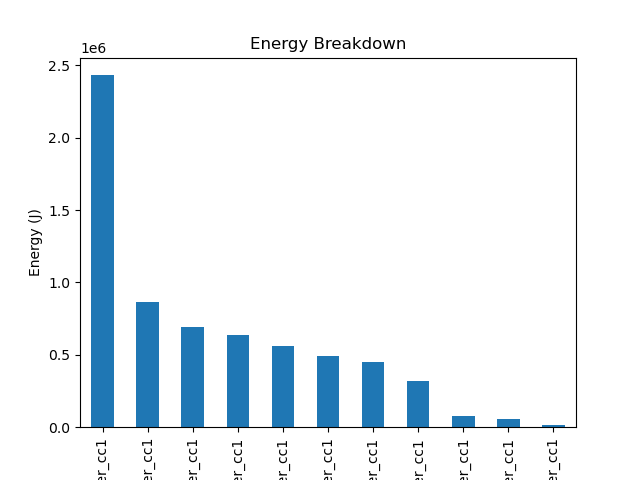
\includegraphics[width=\linewidth]{./assets/energy_breakdown.png}
    \caption{Energy Usage By Component}
    \label{fig:energy_breakdown}
  \end{figure}

  The following sections will go through the various components of the energy consumption, and attempt to optimize them.

  \subsubsection{Clock Power}
  I'm not aware of any parameters we have which directly reduce the overall clock power. Other changes may increase our IPC and therefore reduce the number of cycles, which will be caught by optimising individual components like the functional units or caches.

  \subsubsection{ALU Power}
  The second largest component of energy usage is the ALU, which might be quite a hard one to reduce because the instructions we need to execute are constant, however, we can try changing the number of ALUs we have and see if that makes a difference. While I'm here I will also try changing the number of multipliers and floating point units.

  Doing a parameter search on the number of functional units reveals the only unit that makes any difference is the integer ALU, which is optimal at 2 or 3. This makes sense as the other units are barely used, but the integer ALU is used for random number generation.

  % \begin{figure}[H]
  %   \centering
  %   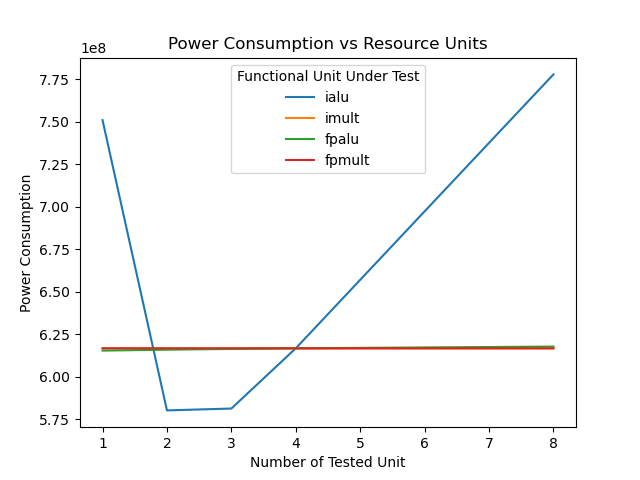
\includegraphics[width=\linewidth]{./assets/units_vs_energy.png}
  %   \caption{Functional Units vs Energy}
  %   \label{fig:units_vs_energy}
  % \end{figure}

  % Figure \ref{fig:units_vs_energy} shows the only functional unit that makes any difference is the integer ALU, which is best at 2. This makes sense as the other units are barely used, but the integer ALU is used for random number generation.

  \optimisation{reduce_ialu}

  I might have expected having unnecessary functional units to increase energy usage, but it seems like SimplerScalar has some mechanism to prevent unused functional units from using energy.

  \subsubsection{L1 Data Cache}
  To optimize L1 cache, I do a 2-way search between cache size and block size.

  \begin{figure}[H]
    \centering
    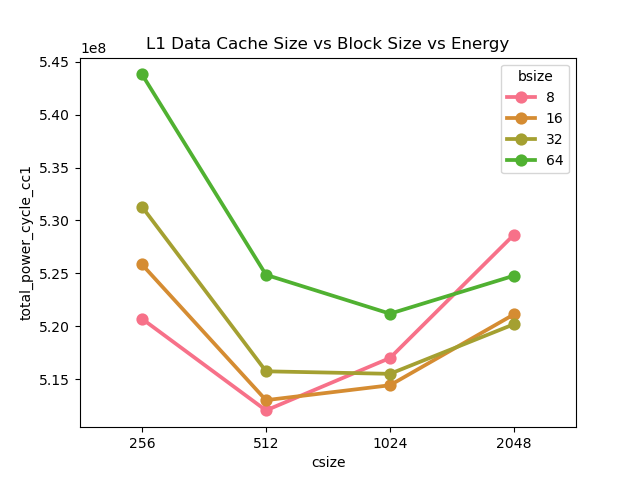
\includegraphics[width=\linewidth]{./assets/l1_vs_energy.png}
    \caption{Block Size \& Cache Size vs Energy}
    \label{fig:l1_vs_energy}
  \end{figure}

  Figure \ref{fig:l1_vs_energy} tells us the optimal cache is 512B large with 16B blocks. I suspected having a small cache would be better due to the temporal locality of splay trees (512B is a 32-fold reduction!) but I don't know why a 16B block performs better than a 32B one.

  Interestingly enough, reducing the cache size does not reduce the requirement for cache, likely because how much cache you need is a function of how far you are likely to step in the random walk, which is controlled by delta and the random number generator, not tree size.

  \optimisation{dl1_cache}

  \subsubsection{L2 (Unified) Cache}
  In SuperScalar, L2 cache seems extremely cheap, so we can fit an enormous amount of the splay tree in it, and prevent the CPU from ever having to go to main memory. To make it prefetch as much as possible, we use a huge block size.

  Figure \ref{fig:l2_vs_energy} shows the optimal for this is having 64KiB of L2 cache with 16KiB blocks.

  \begin{figure}[H]
    \centering
    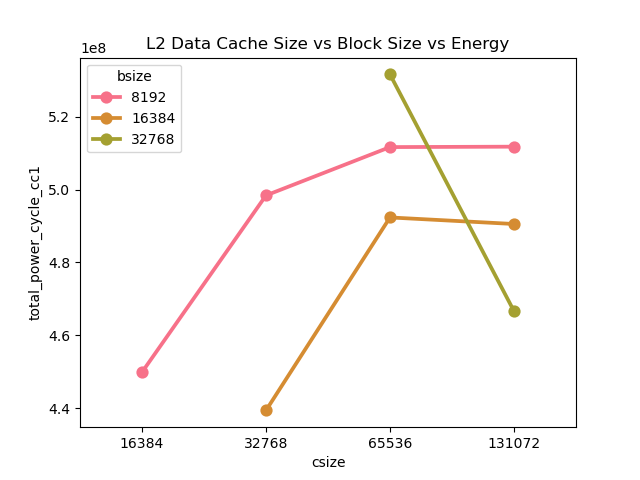
\includegraphics[width=\linewidth]{./assets/l2_vs_energy.png}
    \caption{Energy vs L2 Cache}
    \label{fig:l2_vs_energy}
  \end{figure}

  \optimisation{l2_cache}

  The L1 cache has been drastically shrunk, resulting in nice energy savings.

  \optimisation{il1_cache}

  \subsubsection{Branch Predictor}
  Branch prediction will be important due to the high branching factor of the splay tree program. Trying each predictor individually shows the combined predictor is the best. The optimal meta table size is 16B. Graph omitted for brevity.

  \optimisation{bpred}

  The BTB size can be drastically reduced: as shown in Figure \ref{fig:btb_vs_energy}, the optimal size is 64B with an associativity of 4.

  \begin{figure}[H]
    \centering
    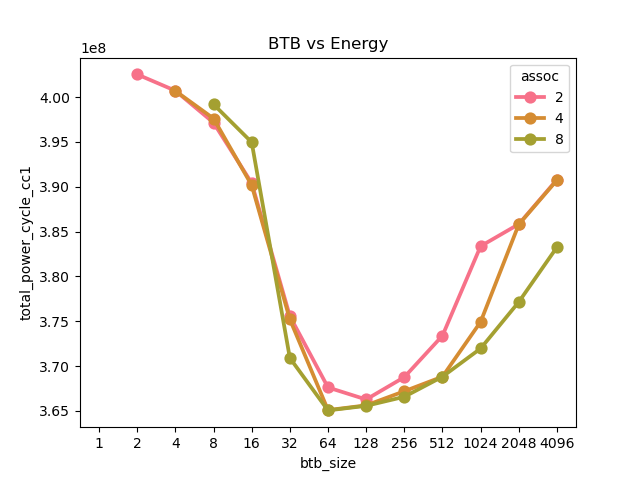
\includegraphics[width=\linewidth]{./assets/btb_vs_energy.png}
    \caption{BTB vs Energy}
    \label{fig:btb_vs_energy}
  \end{figure}

  \optimisation{btb}

  \subsubsection{Issue/Decode/Commit Width}
  While not explicitly an energy-consuming stage, everything is affected by the issue/decode/
  commit width, so I will try to optimize it here. We alter the width of each of these stages individually and see how it affects energy usage.

  \begin{figure}[H]
    \centering
    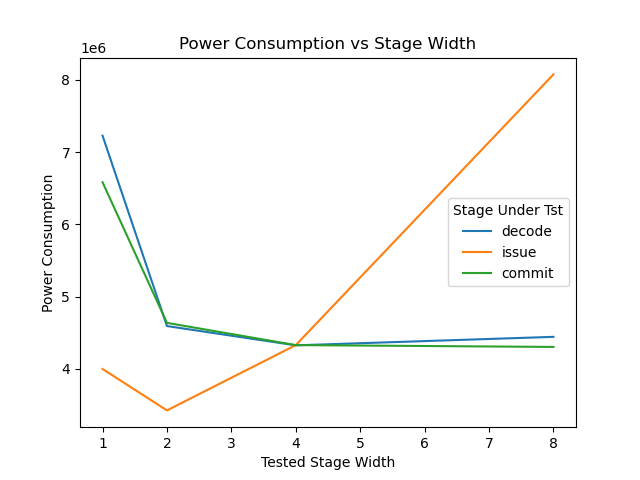
\includegraphics[width=\linewidth]{./assets/width_vs_energy.png}
    \caption{Stage Width vs Energy}
    \label{fig:width_vs_energy}
  \end{figure}

  Figure \ref{fig:width_vs_energy} shows the only improvement from the defaults is setting the issue width to 2. This might help because the high branching factor is causing a lot of pipeline stalls. This makes a huge difference.

  \optimisation{width}

  \subsection{Systematic Optimisation}
  To make sure I'm at a local minimum, I have re-run every experiment in the report so far, starting from the optimal parameters found in the previous section. Now that everything has shrunk, the optimal parameters for the RUU and LSQ are 8 and 4 respectively, as shown by the new version of Figure \ref{fig:energy_vs_ruu_lsq2}.

  \begin{figure}[H]
    \centering
    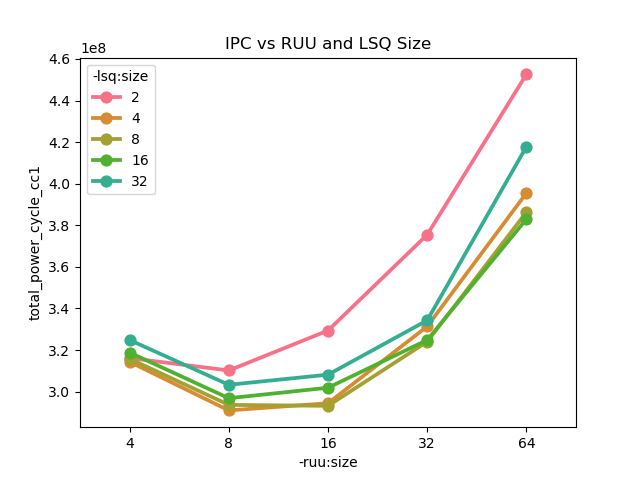
\includegraphics[width=\linewidth]{./assets/energy_vs_ruu_and_lsq_size2.png}
    \caption{Energy vs RUU Size/LSQ Size}
    \label{fig:energy_vs_ruu_lsq2}
  \end{figure}

  \optimisation{ruu_lsq_iter}

  Running all experiments again, no parameters can be improved, therefore we are at a local minimum.

  \subsection{Energy Optimisation Summary}
  After all is said and done, we are down to a very competitive $0.291J$ which is about half the original energy usage. By removing our optimizations one at a time and measuring energy usage, we can see which were most effective.

  \begin{figure}[H]
    \centering
    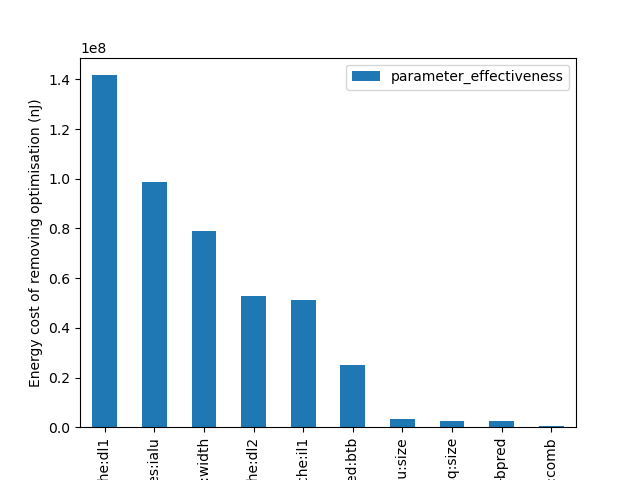
\includegraphics[width=\linewidth]{./assets/parameter_effectiveness.png}
    \caption{Energy Usage Increase Caused By Removing Optimisations}
    \label{fig:parameter_effectiveness}
  \end{figure}

  Figure \ref{fig:parameter_effectiveness} shows the largest improvement by far came from adjusting the caches, of our optimizations 3 are cache-related, including the most effective optimization. They alone account for over half the energy reduction. Final energy = $0.291J$.

  % \begin{tcolorbox}[width=\linewidth, colback=white!95!black, colframe=white!95!black]
  %   \begin{center}\textbf{All Optimizations}\end{center}

  %   \tcblower

  %   Params \hfill \verb|-res:ialu 2|

  %   \hfill \verb|-cache:dl1 dl1:8:16:4:l|

  %   \hfill \verb|-cache:dl2 ul2:1:16384:2:l|

  %   \hfill \verb|-cache:il1 il1:16:64:4:l|

  %   \hfill \verb|-bpred comb|

  %   \hfill \verb|-bpred:comb 16|

  %   \hfill \verb|-bpred:btb 16 4|

  %   \hfill \verb|-issue:width 2|

  %   \hfill \verb|-ruu:size 8|

  %   \hfill \verb|-lsq:size 4|

  %   Energy \hfill \st{$0.617J$} $0.291J$

  % \end{tcolorbox}

\end{multicols}

\end{document}
